% =====================================================================
%  Chapitre 8 : Administration Django
% =====================================================================
\chapter{L'administration Django}
\label{ch:admin}

\chapitreresume{Django fournit une interface d'administration complète, accessible
sans écrire de HTML. Dans ce chapitre, vous créez un superutilisateur, vous
enregistrez les modèles du catalogue, vous personnalisez les listes, les filtres et
les formulaires, puis vous ajoutez des actions de masse et une identité visuelle à
l'interface.}

\begin{objectifs}
\begin{itemize}
  \item Créer un superutilisateur et se connecter à l'administration.
  \item Enregistrer un modèle avec \code{admin.site.register}.
  \item Personnaliser une liste avec \code{ModelAdmin}.
  \item Ajouter des filtres, une recherche, un ordre et une hiérarchie de dates.
  \item Utiliser les inlines pour éditer les objets liés.
  \item Écrire une action personnalisée.
  \item Personnaliser le titre et l'en-tête de l'administration.
  \item Comprendre les limites de sécurité de l'administration.
\end{itemize}
\end{objectifs}

\section{À quoi sert l'administration ?}

L'administration est une application fournie par Django. Elle lit vos modèles et
génère automatiquement des écrans de liste, de création, de modification et de
suppression. Pour un projet de gestion, c'est un gain de temps considérable : les
bibliothécaires peuvent gérer le catalogue avant même que le site public ne soit
terminé.

\begin{retenir}
L'administration n'est pas le site public. C'est un outil interne, réservé aux
personnes autorisées. Les bibliothécaires y ajoutent des livres, corrigent des
fiches et enregistrent des retours. Les lecteurs, eux, utilisent les pages
publiques.
\end{retenir}

L'application d'administration fait partie des applications installées par
défaut. Sa route est déjà branchée dans le fichier d'URL du projet :

\begin{codebox}[python]{gesibiblio/urls.py, extrait}
path("admin/", admin.site.urls),
\end{codebox}

\section{Créer un superutilisateur}

\begin{terminal}
python manage.py createsuperuser
\end{terminal}

Django demande un nom d'utilisateur, une adresse électronique et un mot de passe.
Le mot de passe n'est pas affiché pendant la saisie. Sortie typique :

\begin{terminal}
Nom d'utilisateur : admin
Adresse électronique : admin@gesibiblio.example
Password :
Password (again) :
Superuser created successfully.
\end{terminal}

Lancez le serveur, puis ouvrez \code{http://127.0.0.1:8000/admin/}.

\begin{attention}
Un superutilisateur a tous les droits. Ne partagez pas ce compte, ne le créez pas
avec le mot de passe \code{admin} et ne le laissez pas accessible en production
sans HTTPS. Pour le développement local, un compte simple suffit.
\end{attention}

Au premier démarrage, l'administration ne montre que les groupes et les
utilisateurs. Nos modèles n'apparaissent pas encore : il faut les enregistrer.

\section{Enregistrer les modèles}

Ouvrez \code{catalogue/admin.py}. La forme minimale :

\begin{codebox}[python]{catalogue/admin.py, version minimale}
from django.contrib import admin

from .models import Auteur, Categorie, Emprunt, Livre, Membre

admin.site.register(Auteur)
admin.site.register(Categorie)
admin.site.register(Livre)
admin.site.register(Membre)
admin.site.register(Emprunt)
\end{codebox}

Rechargez la page : les cinq modèles apparaissent dans la section
\og Catalogue \fg. Vous pouvez déjà ajouter un livre.

\begin{figure}[htbp]
\centering
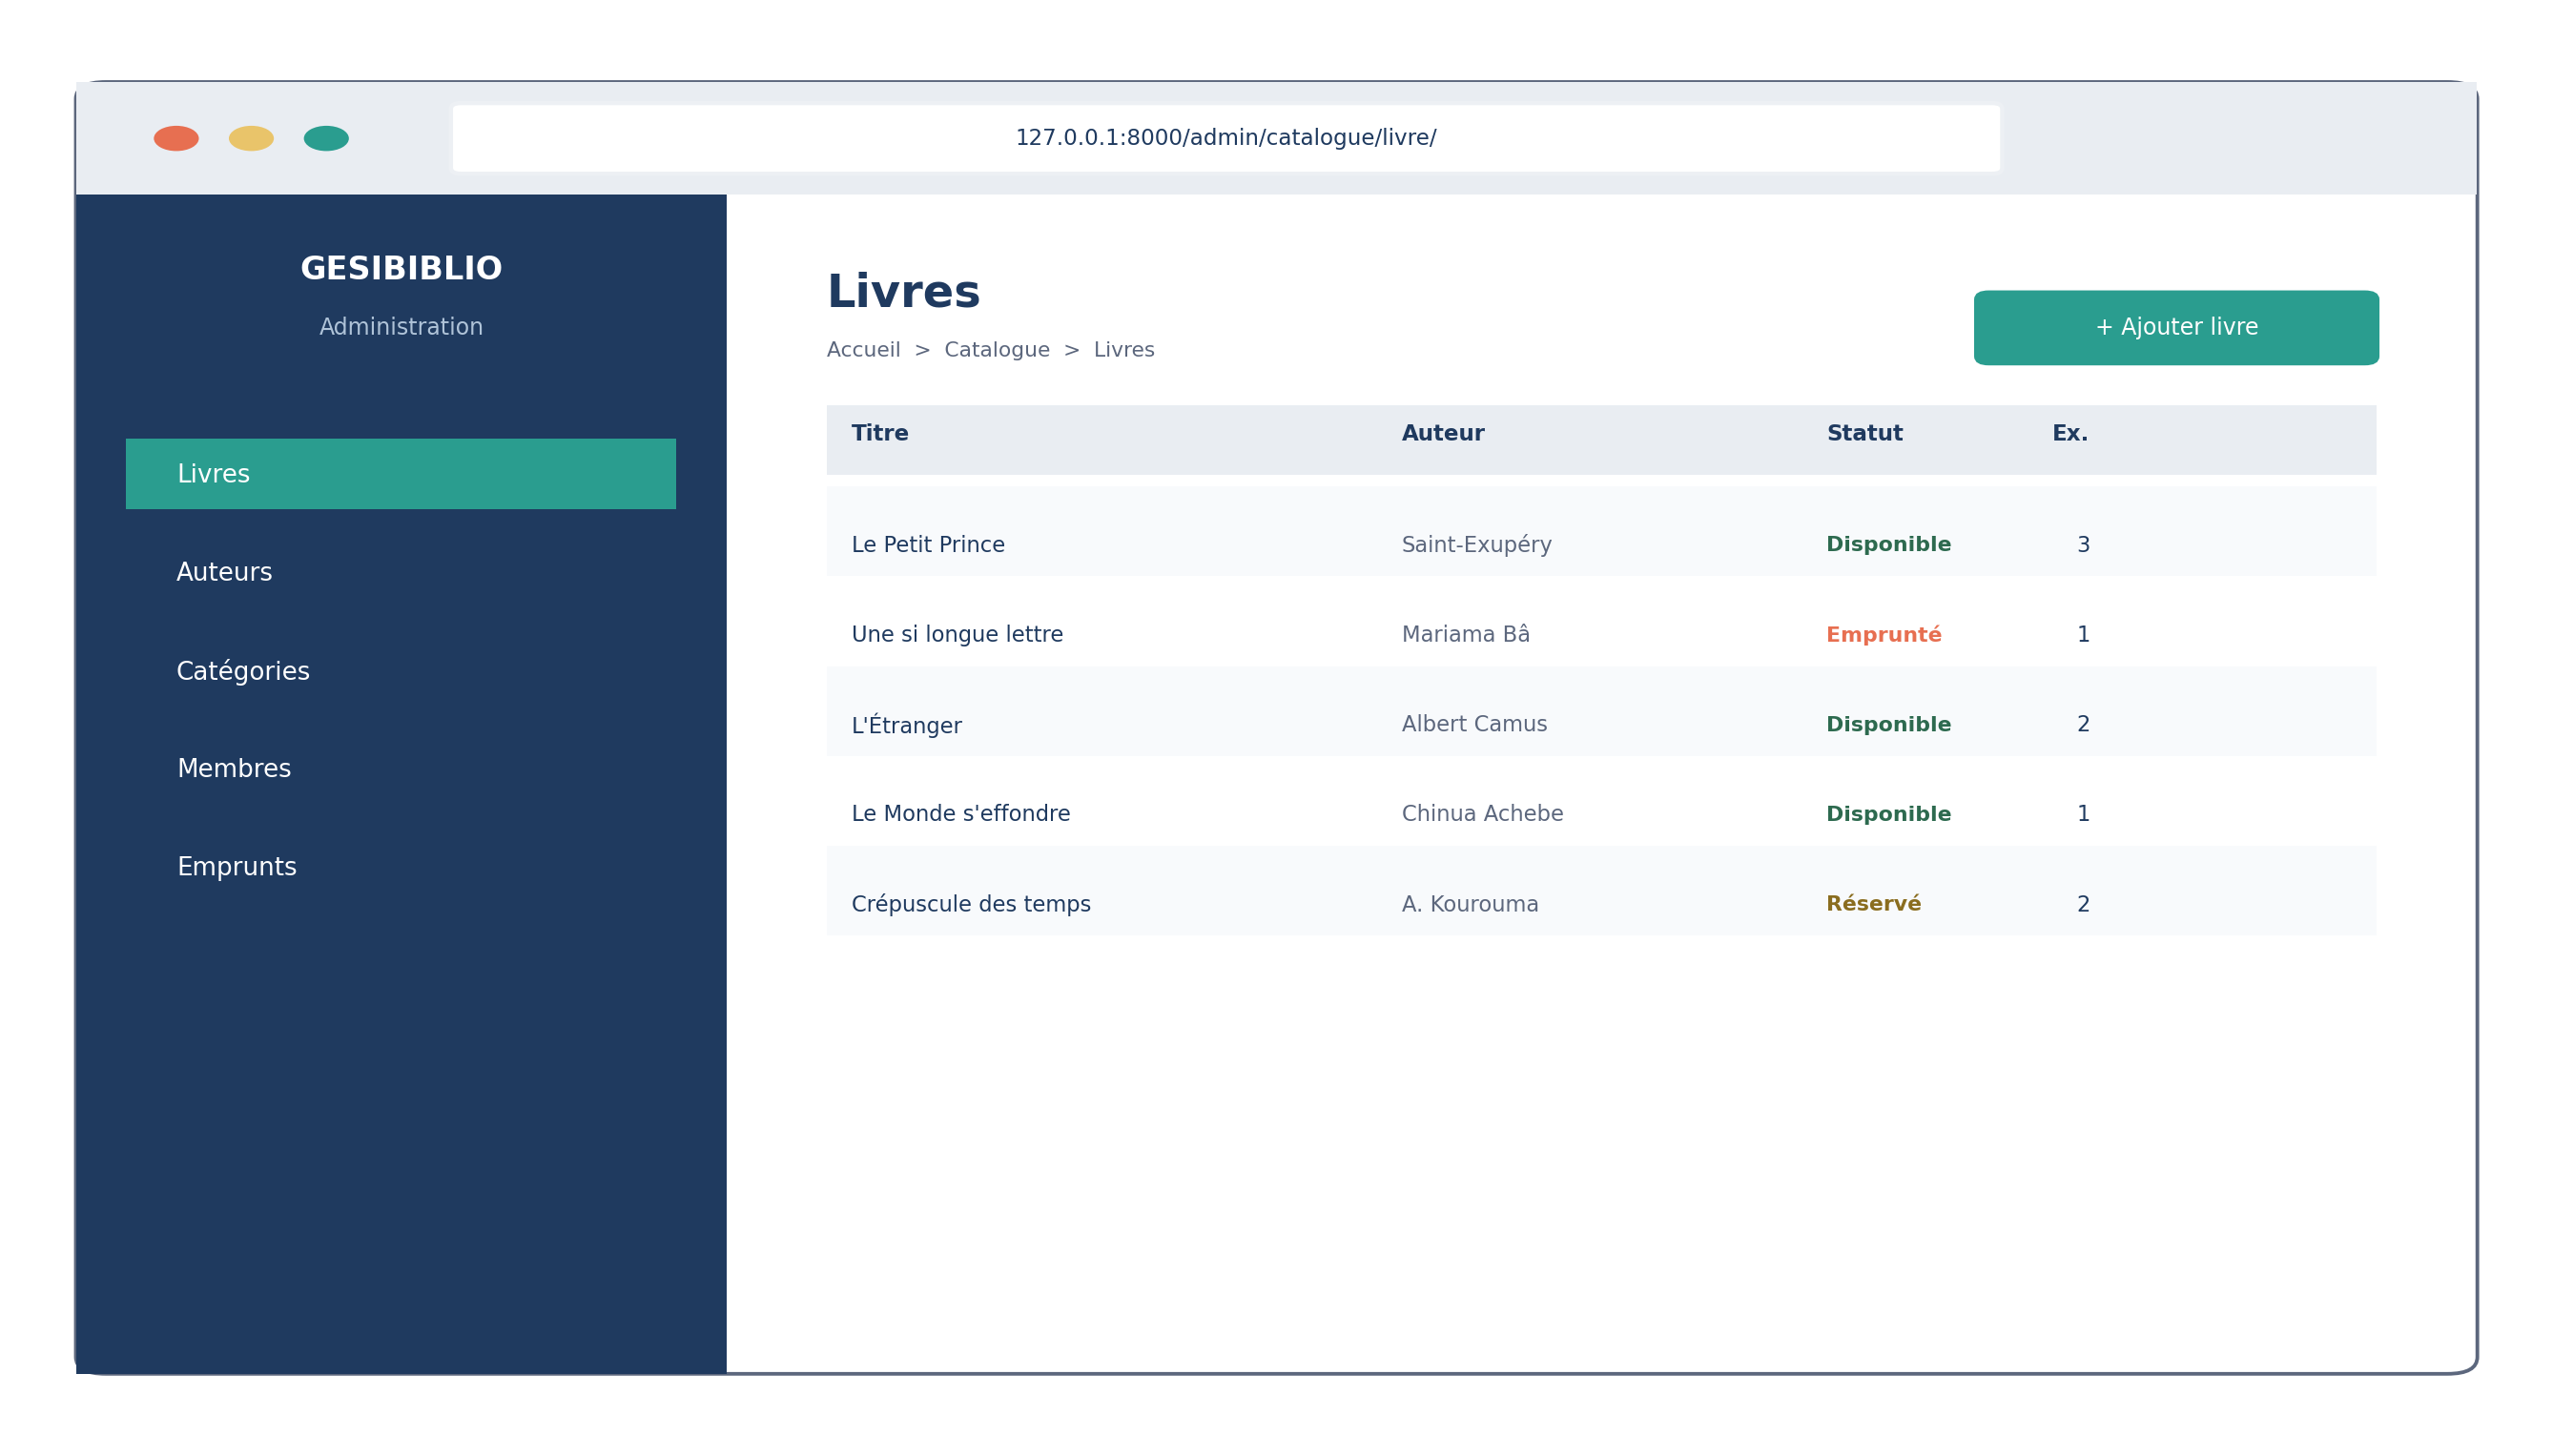
\includegraphics[width=\textwidth]{images/admin_mockup.png}
\caption{La liste des livres dans l'administration, avec les colonnes
personnalisées, les filtres et le bouton d'ajout.}
\label{fig:admin}
\end{figure}

\section{Personnaliser l'affichage}

\code{admin.site.register(Livre)} suffit pour démarrer, mais la liste par défaut
affiche seulement \code{\_\_str\_\_}. Pour un vrai usage, on déclare une classe
\code{ModelAdmin}.

\begin{codebox}[python]{catalogue/admin.py}
from django.contrib import admin

from .models import Auteur, Categorie, Emprunt, Livre, Membre


@admin.register(Auteur)
class AuteurAdmin(admin.ModelAdmin):
    list_display = ("nom", "prenom", "date_naissance", "nb_livres")
    search_fields = ("nom", "prenom")
    ordering = ("nom", "prenom")

    @admin.display(description="Livres")
    def nb_livres(self, obj):
        return obj.livres.count()


@admin.register(Categorie)
class CategorieAdmin(admin.ModelAdmin):
    list_display = ("nom", "slug", "nb_livres")
    search_fields = ("nom",)
    prepopulated_fields = {"slug": ("nom",)}

    @admin.display(description="Livres")
    def nb_livres(self, obj):
        return obj.livres.count()


@admin.register(Livre)
class LivreAdmin(admin.ModelAdmin):
    list_display = (
        "titre",
        "auteur",
        "annee_publication",
        "statut",
        "nombre_exemplaires",
    )
    list_filter = ("statut", "categories", "annee_publication")
    search_fields = ("titre", "isbn", "auteur__nom")
    list_select_related = ("auteur",)
    date_hierarchy = "cree_le"
    ordering = ("titre",)
    readonly_fields = ("cree_le", "modifie_le")
    autocomplete_fields = ("auteur", "categories")
    fieldsets = (
        ("Identification", {
            "fields": ("titre", "sous_titre", "slug", "isbn"),
        }),
        ("Publication", {
            "fields": (
                "auteur",
                "editeur",
                "annee_publication",
                "categories",
            ),
        }),
        ("Stock", {
            "fields": ("nombre_exemplaires", "statut", "couverture"),
        }),
        ("Contenu", {
            "fields": ("resume",),
        }),
        ("Suivi", {
            "fields": ("cree_le", "modifie_le"),
            "classes": ("collapse",),
        }),
    )


@admin.register(Membre)
class MembreAdmin(admin.ModelAdmin):
    list_display = ("numero", "user", "telephone", "actif", "date_inscription")
    list_filter = ("actif",)
    search_fields = ("numero", "user__username", "user__last_name")
    autocomplete_fields = ("user",)
    date_hierarchy = "date_inscription"


@admin.register(Emprunt)
class EmpruntAdmin(admin.ModelAdmin):
    list_display = (
        "livre",
        "membre",
        "date_emprunt",
        "date_retour_prevue",
        "rendu",
        "retard",
    )
    list_filter = ("date_emprunt", "date_retour_prevue")
    search_fields = ("livre__titre", "membre__numero")
    list_select_related = ("livre", "membre")
    date_hierarchy = "date_emprunt"
    autocomplete_fields = ("livre", "membre")

    @admin.display(boolean=True, description="Rendu")
    def rendu(self, obj):
        return obj.date_retour is not None

    @admin.display(boolean=True, description="En retard")
    def retard(self, obj):
        return obj.est_en_retard
\end{codebox}

\begin{attention}
\code{autocomplete\_fields} exige que le modèle cible possède un
\code{search\_fields} dans son \code{ModelAdmin}. Pour \code{livre} et
\code{membre}, c'est le cas. Pour \code{user}, il faut enregistrer un
\code{UserAdmin} personnalisé ou retirer \code{user} de
\code{autocomplete\_fields}.
\end{attention}

\subsection{Les options de liste}

\begin{table}[htbp]
\centering
\small
\begin{tabularx}{\textwidth}{L{5.1cm} X}
\toprule
\textbf{Option} & \textbf{Effet} \\
\midrule
\code{list\_display} & Colonnes affichées. Accepte des noms de champs, des
méthodes et des propriétés. \\
\code{list\_filter} & Filtres dans la barre latérale droite. \\
\code{search\_fields} & Champs interrogés par la recherche. \\
\code{list\_select\_related} & Charge les clés étrangères en une requête. \\
\code{list\_per\_page} & Nombre d'objets par page. \\
\code{ordering} & Ordre par défaut de la liste. \\
\code{date\_hierarchy} & Navigation par année, mois et jour. \\
\code{list\_editable} & Modifie un champ directement dans la liste. \\
\code{list\_display\_links} & Champs cliquables vers la fiche. \\
\bottomrule
\end{tabularx}
\caption{Options principales d'une liste d'administration.}
\end{table}

\begin{bonne}
Ajoutez \code{list\_select\_related} dès que \code{list\_display} contient une clé
étrangère. Sans cela, Django exécute une requête par ligne pour afficher l'auteur
de chaque livre. Sur 500 livres, cela fait 501 requêtes.
\end{bonne}

\subsection{Les colonnes calculées}

\begin{codebox}[python]{Colonne avec décorateur}
@admin.display(description="Livres", ordering="livres__count")
def nb_livres(self, obj):
    return obj.livres.count()
\end{codebox}

\begin{description}[leftmargin=4.4cm,style=nextline]
  \item[\code{description}] Titre de la colonne.
  \item[\code{boolean}] Affiche une icône verte ou rouge.
  \item[\code{ordering}] Permet de trier la colonne. Pour un comptage, la valeur
  doit être une expression acceptée par l'ORM, souvent une annotation.
\end{description}

\begin{note}
Une colonne calculée avec \code{obj.livres.count()} déclenche une requête par
ligne. Pour une liste volumineuse, annotez le queryset dans
\code{get\_queryset()} avec \code{Count("livres")} et lisez l'attribut ajouté.
\end{note}

\section{Les formulaires d'administration}

\subsection{fieldsets}

\code{fieldsets} regroupe les champs en sections. Chaque section est un couple
\og titre, dictionnaire \fg. Le dictionnaire contient \code{fields} et
éventuellement \code{classes} (\code{collapse}, \code{wide}).

\begin{codebox}[python]{fieldsets, extrait}
fieldsets = (
    ("Identification", {
        "fields": ("titre", "isbn"),
    }),
    ("Détails", {
        "fields": ("auteur", "annee_publication"),
        "classes": ("collapse",),
    }),
)
\end{codebox}

\begin{attention}
Si vous utilisez \code{fieldsets}, tous les champs éditables doivent y figurer.
Un champ oublié disparaît du formulaire et devient impossible à modifier. Les
champs \code{readonly\_fields} doivent aussi être listés.
\end{attention}

\subsection{prepopulated\_fields}

\begin{codebox}[python]{Slug automatique}
prepopulated_fields = {"slug": ("titre",)}
\end{codebox}

Le slug se remplit pendant la saisie du titre, en JavaScript. L'utilisateur peut le
corriger. C'est un confort, pas une validation : le modèle garde
\code{unique=True}.

\subsection{Les inlines}

Un emprunt appartient à un livre et à un membre. Pour voir les emprunts d'un livre
directement dans sa fiche, on utilise un inline.

\begin{codebox}[python]{Inline d'emprunts}
class EmpruntInline(admin.TabularInline):
    model = Emprunt
    extra = 1
    fields = ("membre", "date_emprunt", "date_retour_prevue", "date_retour")
    autocomplete_fields = ("membre",)


@admin.register(Livre)
class LivreAdmin(admin.ModelAdmin):
    # ... options existantes
    inlines = [EmpruntInline]
\end{codebox}

\begin{description}[leftmargin=3.6cm,style=nextline]
  \item[\code{TabularInline}] Tableau compact, adapté aux relations simples.
  \item[\code{StackedInline}] Formulaire vertical, adapté aux objets riches.
  \item[\code{extra}] Nombre de lignes vides proposées.
  \item[\code{can\_delete}] Autorise la suppression des lignes liées.
\end{description}

\begin{attention}
Un inline ne fonctionne que si la clé étrangère pointe vers le modèle parent. Ici,
\code{Emprunt.livre} pointe vers \code{Livre}. Pour une relation
plusieurs à plusieurs, utilisez \code{filter\_horizontal} ou
\code{autocomplete\_fields}, pas un inline.
\end{attention}

\section{Les actions de masse}

Une action s'applique à plusieurs objets sélectionnés. Exemple : marquer des livres
comme perdus, ou exporter une sélection en CSV.

\begin{codebox}[python]{catalogue/admin.py, extrait}
import csv

from django.http import HttpResponse


@admin.action(description="Marquer les livres sélectionnés comme perdus")
def marquer_perdus(modeladmin, request, queryset):
    nombre = queryset.update(statut=Livre.Statut.PERDU)
    modeladmin.message_user(
        request,
        f"{nombre} livre(s) marqué(s) comme perdus.",
    )


@admin.action(description="Exporter la sélection en CSV")
def exporter_csv(modeladmin, request, queryset):
    response = HttpResponse(content_type="text/csv")
    response["Content-Disposition"] = 'attachment; filename="livres.csv"'
    writer = csv.writer(response)
    writer.writerow(["Titre", "Auteur", "ISBN", "Année", "Statut"])
    for livre in queryset.select_related("auteur"):
        writer.writerow([
            livre.titre,
            livre.auteur,
            livre.isbn,
            livre.annee_publication,
            livre.get_statut_display(),
        ])
    return response


@admin.register(Livre)
class LivreAdmin(admin.ModelAdmin):
    # ... options existantes
    actions = [marquer_perdus, exporter_csv]
\end{codebox}

\begin{bonne}
Les actions doivent être idempotentes autant que possible : les exécuter deux fois
ne doit pas produire de dégât. Affichez toujours un message avec
\code{message\_user} pour indiquer ce qui a été fait. Pour une action destructrice,
ajoutez une page de confirmation.
\end{bonne}

\begin{piege}
Une action qui renvoie \code{None} recharge la liste. Une action qui renvoie une
\code{HttpResponse} affiche cette réponse : c'est ce que fait l'export CSV. Si
vous oubliez de renvoyer la réponse, le fichier n'est jamais téléchargé.
\end{piege}

\section{Personnaliser l'identité de l'administration}

\begin{codebox}[python]{catalogue/admin.py, extrait}
admin.site.site_header = "GesiBiblio, administration"
admin.site.site_title = "GesiBiblio"
admin.site.index_title = "Gestion de la bibliothèque"
\end{codebox}

On peut aussi changer l'ordre des applications et des modèles :

\begin{codebox}[python]{catalogue/apps.py}
from django.apps import AppConfig


class CatalogueConfig(AppConfig):
    default_auto_field = "django.db.models.BigAutoField"
    name = "catalogue"
    verbose_name = "Catalogue"
\end{codebox}

Le \code{verbose\_name} de l'application et des modèles rend l'interface lisible en
français.

\section{Sécurité de l'administration}

L'administration est puissante. Quelques règles :

\begin{bonne}
\begin{itemize}
  \item utiliser HTTPS en production ;
  \item changer l'URL \code{/admin/} par un chemin moins évident, sans compter
        sur le secret ;
  \item limiter les comptes \code{is\_superuser} ;
  \item donner aux bibliothécaires des permissions précises plutôt qu'un statut
        global ;
  \item activer la double authentification si l'infrastructure le permet ;
  \item sauvegarder la base avant toute opération de masse.
\end{itemize}
\end{bonne}

\begin{attention}
Changer l'URL de l'administration ne remplace pas les permissions. Un attaquant
peut découvrir le chemin. La vraie protection repose sur des mots de passe solides,
HTTPS, des droits limités et une surveillance des connexions.
\end{attention}

\section{Exercices}

\begin{exercice}[ : colonne disponible]
Ajoutez une colonne \og Disponible \fg{} dans la liste des livres. Elle doit
afficher une icône verte si \code{livre.est\_disponible} est vrai, rouge sinon.
\end{exercice}

\begin{correction}
\begin{codebox}[python]{catalogue/admin.py, extrait}
@admin.display(boolean=True, description="Disponible")
def disponible(self, obj):
    return obj.est_disponible
\end{codebox}

Ajoutez \code{"disponible"} à \code{list\_display}. Attention : la propriété
déclenche une requête par livre. Pour une liste courte, c'est acceptable ; pour une
liste longue, annotez le queryset.
\end{correction}

\begin{exercice}[ : filtre personnalisé]
Créez un filtre \code{EmpruntEnRetardFilter} qui affiche seulement les emprunts
dont la date de retour prévue est dépassée et qui ne sont pas rendus.
\end{exercice}

\begin{correction}
\begin{codebox}[python]{catalogue/admin.py, extrait}
from django.utils import timezone


class EmpruntEnRetardFilter(admin.SimpleListFilter):
    title = "emprunts en retard"
    parameter_name = "retard"

    def lookups(self, request, model_admin):
        return (
            ("oui", "En retard"),
            ("non", "À jour"),
        )

    def queryset(self, request, queryset):
        aujourdhui = timezone.localdate()
        if self.value() == "oui":
            return queryset.filter(
                date_retour__isnull=True,
                date_retour_prevue__lt=aujourdhui,
            )
        if self.value() == "non":
            return queryset.filter(
                date_retour__isnull=True,
                date_retour_prevue__gte=aujourdhui,
            )
        return queryset
\end{codebox}

Ajoutez \code{EmpruntEnRetardFilter} à \code{list\_filter}.
\end{correction}

\begin{exercice}[ : recherche par numéro]
Dans l'administration des emprunts, permettez la recherche par numéro de membre et
par titre de livre. Vérifiez que la recherche fonctionne avec les deux.
\end{exercice}

\begin{correction}
\begin{codebox}[python]{catalogue/admin.py, extrait}
search_fields = ("livre__titre", "membre__numero")
\end{codebox}

La double barre basse traverse la relation. Django construit la jointure
nécessaire. Vérifiez que \code{Membre.\_\_str\_\_} affiche le numéro pour rendre le
résultat lisible.
\end{correction}

\begin{retenir}
\begin{itemize}
  \item \code{createsuperuser} crée un compte administrateur.
  \item \code{admin.site.register} rend un modèle visible.
  \item \code{ModelAdmin} personnalise la liste et le formulaire.
  \item \code{list\_select\_related} évite le problème N+1.
  \item Les inlines éditent les objets liés dans la fiche parente.
  \item Les actions de masse agissent sur une sélection.
  \item L'administration est un outil interne : protégez-la.
\end{itemize}
\end{retenir}
